\section{Detection \& Eviction}
\label{sec:detection}

In this section, we describe the main building blocks that constitutes proposed detection mechanism that targets detecting malicious peers in order to restore benign peers satisfaction.
We start by discussing the main differences between detecting a dropping attack behavior and detecting a manipulation/outdated chunks attack behavior, referred to as \textit{drop} attack, \textit{manp} attack for simplicity.
Afterwards, each detection sub-block, as illustrated in Figure~\ref{detection-blocks}, is described.
The list of variables used throughout the paper is provided in Table \ref{tab:acronyms}.

\begin{table}[ht]
\center
\caption{Acronyms}
\begin{tabular}{|c|l||c|l|}
\hline

\bf{Var.} & \bf{Description}  & \bf{Var.} & \bf{Description} \\\hline\hline
$x$ & no. of malicious peers & $\eta$ & fraction of mal. headnodes\\\hline
$MN$ & malicious neighbors & $\sigma$ & satisfaction threshold\\\hline
$H_n$ & list of headnodes & $P_n$ & list of potential candidates \\\hline
$\alpha$ & manipulation threshold& $F$ & familiarity of suspect \\\hline
$G$ & suspect guilt value & $\kappa$ & dropping det. allowed\\\hline
$NL$ & neighbor list & $BM$ & buffer map\\\hline
\end{tabular}
\label{tab:acronyms}
\end{table}

\subsection{Drop vs. Manp Detection}
On one hand, when $m$ conducts a drop attack on $b$, $b$ is not capable of detecting any malicious behavior.
Specifically, in a drop attack, $m$ never sends the actual $BM$ that represents the chunks it currently acquires.
Hence, $m$ appears as unsatisfied benign peer to $b$.
In turn, while $b$ is still unsatisfied, it can not detect a certain suspect. 

On the other hand, in a manipulation or outdated chunks, $m$ indeed is eventually suspected to be malicious as $b$ already expects the requested chunk to be sent from $m$ as $m$ claimed.
Thus, eventually $b$ can suspect $m$ as being malicious.
To that end, through the rest of the section, we describe how the detection mechanism handles the aforementioned cases separately.

\begin{figure}
 \centering
 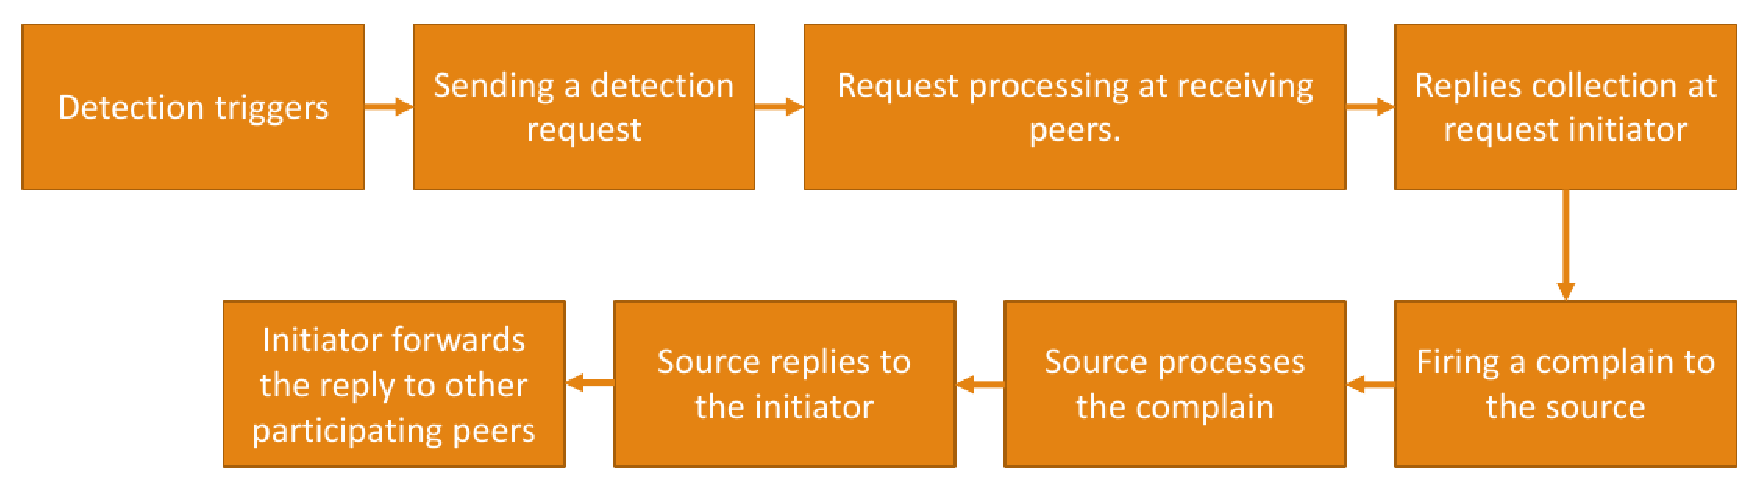
\includegraphics[width=8cm,height=3cm]{./Figures/detection-blocks.eps}
  \caption{Detection mechanism main blocks}
\label{detection-blocks} 
\end{figure}

\subsection{Detection Trigger}
Here we describe how a peer decides on sending a detection request for both attack behaviors.
In both cases, once $b$ decides on sending a detection request, it only send it to peers in its own neighbor list $NL$ to check if those neighbors agree with it or not, disregarding the source if $b$ is a headnode.

Afterwards, as detailed in Section~\ref{Firing_a_Complain}, once $b$ receives its neighbors replies to the detection request, $b$ decides whether or not to fire a complain to the source.
We assume that the source's address is publicly known and any peer can send a complain to the source directly whether the source is already a neighbor to this peer or not.
\subsubsection*{Drop trigger}
In this, as there is no evidence of a manipulation from any neighbor to $b$, the only factor that $b$ is concerned about is the satisfaction threshold $\sigma$.
In details, $b$ decides to trigger a detection request only if:
\begin{enumerate}
 \item $b$'s instant $satisfaction level < \sigma$.
 \item Number of drop detections sent by $b$ in the last $1000s$ is $< \kappa$.
\end{enumerate}
The latter condition guarantees that any peer can not trigger multiple detection requests in parallel so that: (a) to avoid exhausting the source's bandwidth, and (b) the source is most likely processing another peer's dropping request that might eventually positively impact $b$'s satisfaction level.

\subsubsection*{Manp trigger}
$b$ decides to send a detection request if it was manipulated $\alpha$ times by $m$.
This condition essentially guarantees that any peer is not suspected instantly if it did not deliver the requested chunk, i.e., a benign peer might not deliver a chunk to the requester if it is already loaded serving other peers.

In order to avoid malicious peers from abusing the manipulation detection mechanism, $b$ informs $m$ when $\alpha_m = \alpha -1$.
Accordingly, $m$ should give highest priority to $b$ and send the requested chunk signed and waits for a signed Ack from $b$ as an evidence for not manipulating.
This evidence is later needed for the source to decide about $m$.

\subsection{Processing Detection Request}

\subsection{Firing a Complain}
\label{sec:Firing_a_Complain}

\subsection{Processing a Complain at the Source}

\subsection{Processing a Complain Reply \& Forwarding}







